\section{Attacks on Hardware}
\red{ make this flow with previous paragraphs. make sure you mention that you have to know what chip you are trying to reverse (\citep{sergei:thesis} and hardware reveng course). for chemicals see for delayering see :http://siliconpr0n.org/wiki/doku.php?id=chemical:start ,  http://siliconpr0n.org/wiki/doku.php?id=delayer:start  }
\label{sec:curr_attacks}
A distinction between \emph{passive} and \emph{active} attacks should be made. In the former the attacker simply monitors the chip's normal operation and tries to infer the input-output mapping whereas in the latter case the attacker actively manipulates either the chip or its operating environment with the aim of obtaining insight on the chips inner workings. 

Attacks on MCUs may attempt to recover a number of artefacts, including cryptographic keys the and firmware and do not need to necessarily attack the hardware itself but can exploit flaws in algorithmic design and implementation and protocol failures or inter-component communication patterns\citep{anderson:cautionary_note}\citep{kocher:DPA}, obtain information by corrupting the memory or exploiting memory remanence\citep{sergei:thesis}\citep{gutman:memory_remanence}.

The following discussion closely follows \citep{sergei:thesis}.

	\subsection{Non-Invasive Attacks}
	\red{mention other non-invassive attacks as well and SCA, such as exposure to abnormal temperatures, exposure to radiation or using lasers damage/alter/heat specific portions of the chip. make this more technical. \citep{website:riscure}}
	Non-invasive attacks are attacks which require no depackaging or special preparation of the chip and hence attacks under this category leave little tamper evidence behind. These attacks might be very time consuming to find and are not guaranteed to be successful, but are very easy and cheap to replicate once found. Furthermore, non-invasive attacks could target badly implemented communication, bugs or security protocols in order to bypass security restrictions.
	
	\subsubsection{Power Analysis}
	\red{ need sampling equipment with at least double the operating frequency to get a measurement per clock cycle  and also check out Correlational Power Analysis \citep{DPA}\citep{website:riscure}  . could also include image from DPA paper showing DES rounds. also say set up, how and where you place the resistors. see DPA paper again. Also mention EM radiation detection.}
	
	\label{subsubsec:power_analysis}

	\begin{figure}
		\center
		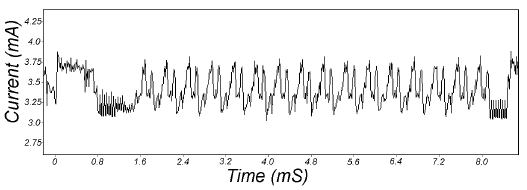
\includegraphics[scale=0.7]{img/power_des.png}
		\caption{\footnotesize Power trace during a DES encryption, where the 16 rounds are clearly visible.(source: \protect\citep{kocher:DPA}).}
		\label{fig:des_power}		
	\end{figure}

	Different instructions executing on a CPU require different amounts of power \citep{website:riscure}\citep{kocher:DPA}, and hence one can infer which instruction is executing on a CPU by analysing a power trace generated by the MCU. These attacks are easy and relatively inexpensive to perform as they only require widely available tools.
	
	Simple Power Analysis(SPA) involves direct observation of the MCU when it performs cryptographic operations and can leak information about both the keys and the cryptographic operations themselves (i.e. nature or structure of the algorithm)\citep{kocher:DPA}\citep{anderson:tamper_resistance}. 

	Differential Power Analysis(DPA) extracts sensitive information by using statistical techniques on very large traces. The techniques involves obtaining power traces of known cipher-texts(but not necessarily knowing the corresponding plain-texts) and individual bits of the key are recovered by analysing the differences in power consumption\citep{kocher:DPA}\citep{anderson:tamper_resistance}.
	
	One can generally avoid noise in their power measurements by sampling the voltage (usually) on the ground line\citep{sergei:thesis}.

	\subsubsection{Glitch and Fault Injection Attacks}
	Glitches and faults are achieved by exposing the device in operating conditions that it was not meant to operate in and attempt to exploit undefined behaviour of the MCU\citep{sergei:thesis}\citep{avr_mega}. Although inducing a fault is easy, inducing an exploitable fault is hard but can be achieved by systematic search {sergei:thesis}\citep{glitches_paper}\citep{website:riscure}.
	
		\emph{Power glitches} and \emph{clock glitches} aim to make the CPU skip or execute incorrect instructions by applying transients. This attack can target in individual components of an MCU and a systematic search can deduce which components are affected by a given glitch sequence. Clock glitches involve increasing the clock signal frequency so that some flip flops sample their input before being updated and hence report an incorrect value. Clock glitches are mainly aimed against software-based protection mechanisms, affecting CPU operation by supplying the CPU with incorrect data.	Power glitches work by supplying either too much power or too little, shifting transistors' threshold and causing flip-flops to read their state incorrectly. Power glitches need to be carefully synchronised with the internal clock and prolonged attacks might damage the board. Glitch attacks are especially dangerous as they may abuse the program counter in order to map out the memory\citep{glitches_paper}\citep{anderson:cautionary_note}\citep{sergei:thesis}.

	\begin{figure}
		\center
		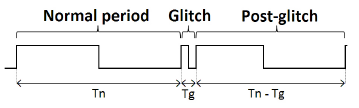
\includegraphics[scale=0.7]{img/clock_glitch.png}
		\caption{\footnotesize Illustration of the principle of a clock-glitch attack.(source: \protect\citep{glitches_paper}).}
		\label{fig:glitch}		
	\end{figure}

	\subsubsection{Data Remanence}
	{\color{red} explain more, make more technical. also cite \citep{website:ibm_secure} who also talks about memory remanence}
	Prolonged exposure of SRAM cells to the same values can make the cells 'remember' their state, due to material properties and stress\citep{gutman:memory_remanence}. Furthermore, cooling the memory down can prolong the time for the data to leave the memory \citep{gutman:memory_remanence}\citep{sergei:RAM}\citep{sergei:thesis}. If, for example, a start-up routine always writes security keys to the same memory location, after some time they key will be recoverable by looking at the physical state of the memory or by cooling down the chip, starting it and then reading the memory.
	
	EEPROM suffers as well, but to a lesser extent, as material-wise one can only tell virgin-cells from used cells\citep{sergei:thesis}. 
	
	\subsubsection{Timing Attacks}
	Timing attacks exploit the software implementation of cryptographic algorithms. Compiler optimisations (avoiding unnecessary branches, register and cache usage) and other implementation choices make the execution time of an algorithm dependent on the input and the secret key, rather being fixed for any input. For example, when input is compared byte-wise with a key and rejected when the first non-matching byte is found, rather than first consuming the whole input string.
	
	Different instructions take different time to execute(e.g. \texttt{MOV eax,[eax]} is considerably slower than \texttt{INC eax}) and thus one could collect timing information for various input messages and systematically deduce the correct key. 
	
	If timing information is correlated with power analysis then defences such as constant instruction execution time could be defeated. One might use \texttt{NOP}s in the case of a wrong key in order for rejection and confirmation responses to have constant execution time but \texttt{NOP} consumes substantially less power than \texttt{INC eax} and correlating timing and power consumption information would reveal this.

	\subsection{Semi-Invasive Attacks}
	Semi-invasive attacks require depackaging of the chip but do not destroy the passivation layer as no electrical contact with the chip is needed. Semi-invasive attacks can be automated and can yield results faster and cheaper than invasive attacks.
	
	\subsubsection{UV Light Exposure}
	Older chips and chips that are designed to withstand low-cost non-invasive (i.e. no depackaging) attacks are susceptible to having parts of the memory altered if it is exposed under UV light. Security fuses that prevent read-back of the memory could have their state reset by sufficient exposure under UV light. The attacker must locate the security fuse though, which can be very tricky. 

	\subsubsection{Imaging Attacks}
	Backside imaging involves shining IR light on the rear side of the chip and imaging it from this angle, since it is a mirror-image of the front side. This is possible because, usually, light shown through the backside does not have to go though multiple layers and hence protective metal meshes(discussed in Section~\ref{sec:defenses}) or normal chip layers are avoided. On some chips it is possible to extract ROM contents via this technique by directly observing the memory. An alternative to IR light would be the use of lasers for imaging. Optical Beam Induced Current and Light Induced Voltage Alteration are the two most common techniques for failure analysis that take advantage of the photoelectric effect. These techniques involve shining lasers on the semiconductor surface in order to alter some property; in OBIC a slight current is created and by analysing this one can deduce the device's properties (including defects and anomalies) and produce an image of the the board being scanned, while in LIVA the board is connected to constant power supply and changes in the power supply are monitored as laser is shone on the device, allowing one to deduce the device's characteristics and construct an image\citep{cole:OBIC}. Lasers can also be used to read the state of memory cells in CMOS SRAM\citep{sergei:thesis}.
	
	\subsection{Invasive Attacks}
	Invasive attacks require direct access to the board's surface and as a result destroy the packaging in the process, therefore leaving tamper evidence\citep{sergei:thesis}\citep{hwre}. Invasive attacks usually aim to understand how a MCU works and then develop cheaper non-invasive or semi-invasive attacks for that chip, as invasive attacks are laborious, require expensive equipment and highly skilled attackers\citep{sergei:thesis}.
	
	\paragraph{Exposing the die surface} This usually involves destroying the packaging by using chemicals or drilling(or other methods). While this is a process that is not very complicated\citep{sergei:thesis}, one might have trouble finding the chemicals required. An alternative for depackaging the chip is to send it to a failure analysis lab\citep{website:hacking_the_pic}.
	
	\paragraph{Reverse engineering} both hardware and the software. Hardware reverse engineering requires using reflected light microscopes or SEM (Scanning Electron Microscope) for constructing a complete image of the surface. \red{maybe present layer removal techniques}Layer removal might be required if deeper layers are not visible in order to have a complete view of the device. Software reverse engineering can be accomplished when one has obtained access to the memory.
	
	\paragraph{Micro-probing and Modification} \red{\citep{low_cost_probing} estimate around \$2000 for optical microscope + micropositioners + moving base + electronics , \citep{sergei:thesis} estimates about the same. }In micro-probing sub-micrometer thickness probes are used to establish contact with the bus lines in order to observe and manipulate bus signals. To achieve reliable results a micro-probing workstation\footnote{all moving components should have micrometer precision\red{provide citation}} is used, consisting of a microscope, micro-positioners for the probes, a movable base and a test socket to place the chip. In order to establish contact with the bus lines the passivation layer should be removed, usually done with UV or green lasers, and access to bus lines of deeper layers can be achieved by using a FIB workstation.
	
	Modifications to the MCU's components (adding new interconnects or destroying circuits) are not always necessary, but could prove useful\citep{anderson:tamper_resistance}. For chip modifications to be successful, the attacker must be sophisticated and must have at least partially reverse-engineered the board.
